\documentclass[crop,tikz]{standalone}
\usetikzlibrary{positioning}
\usepackage{amsmath}
\usepackage{physics}

\begin{document}
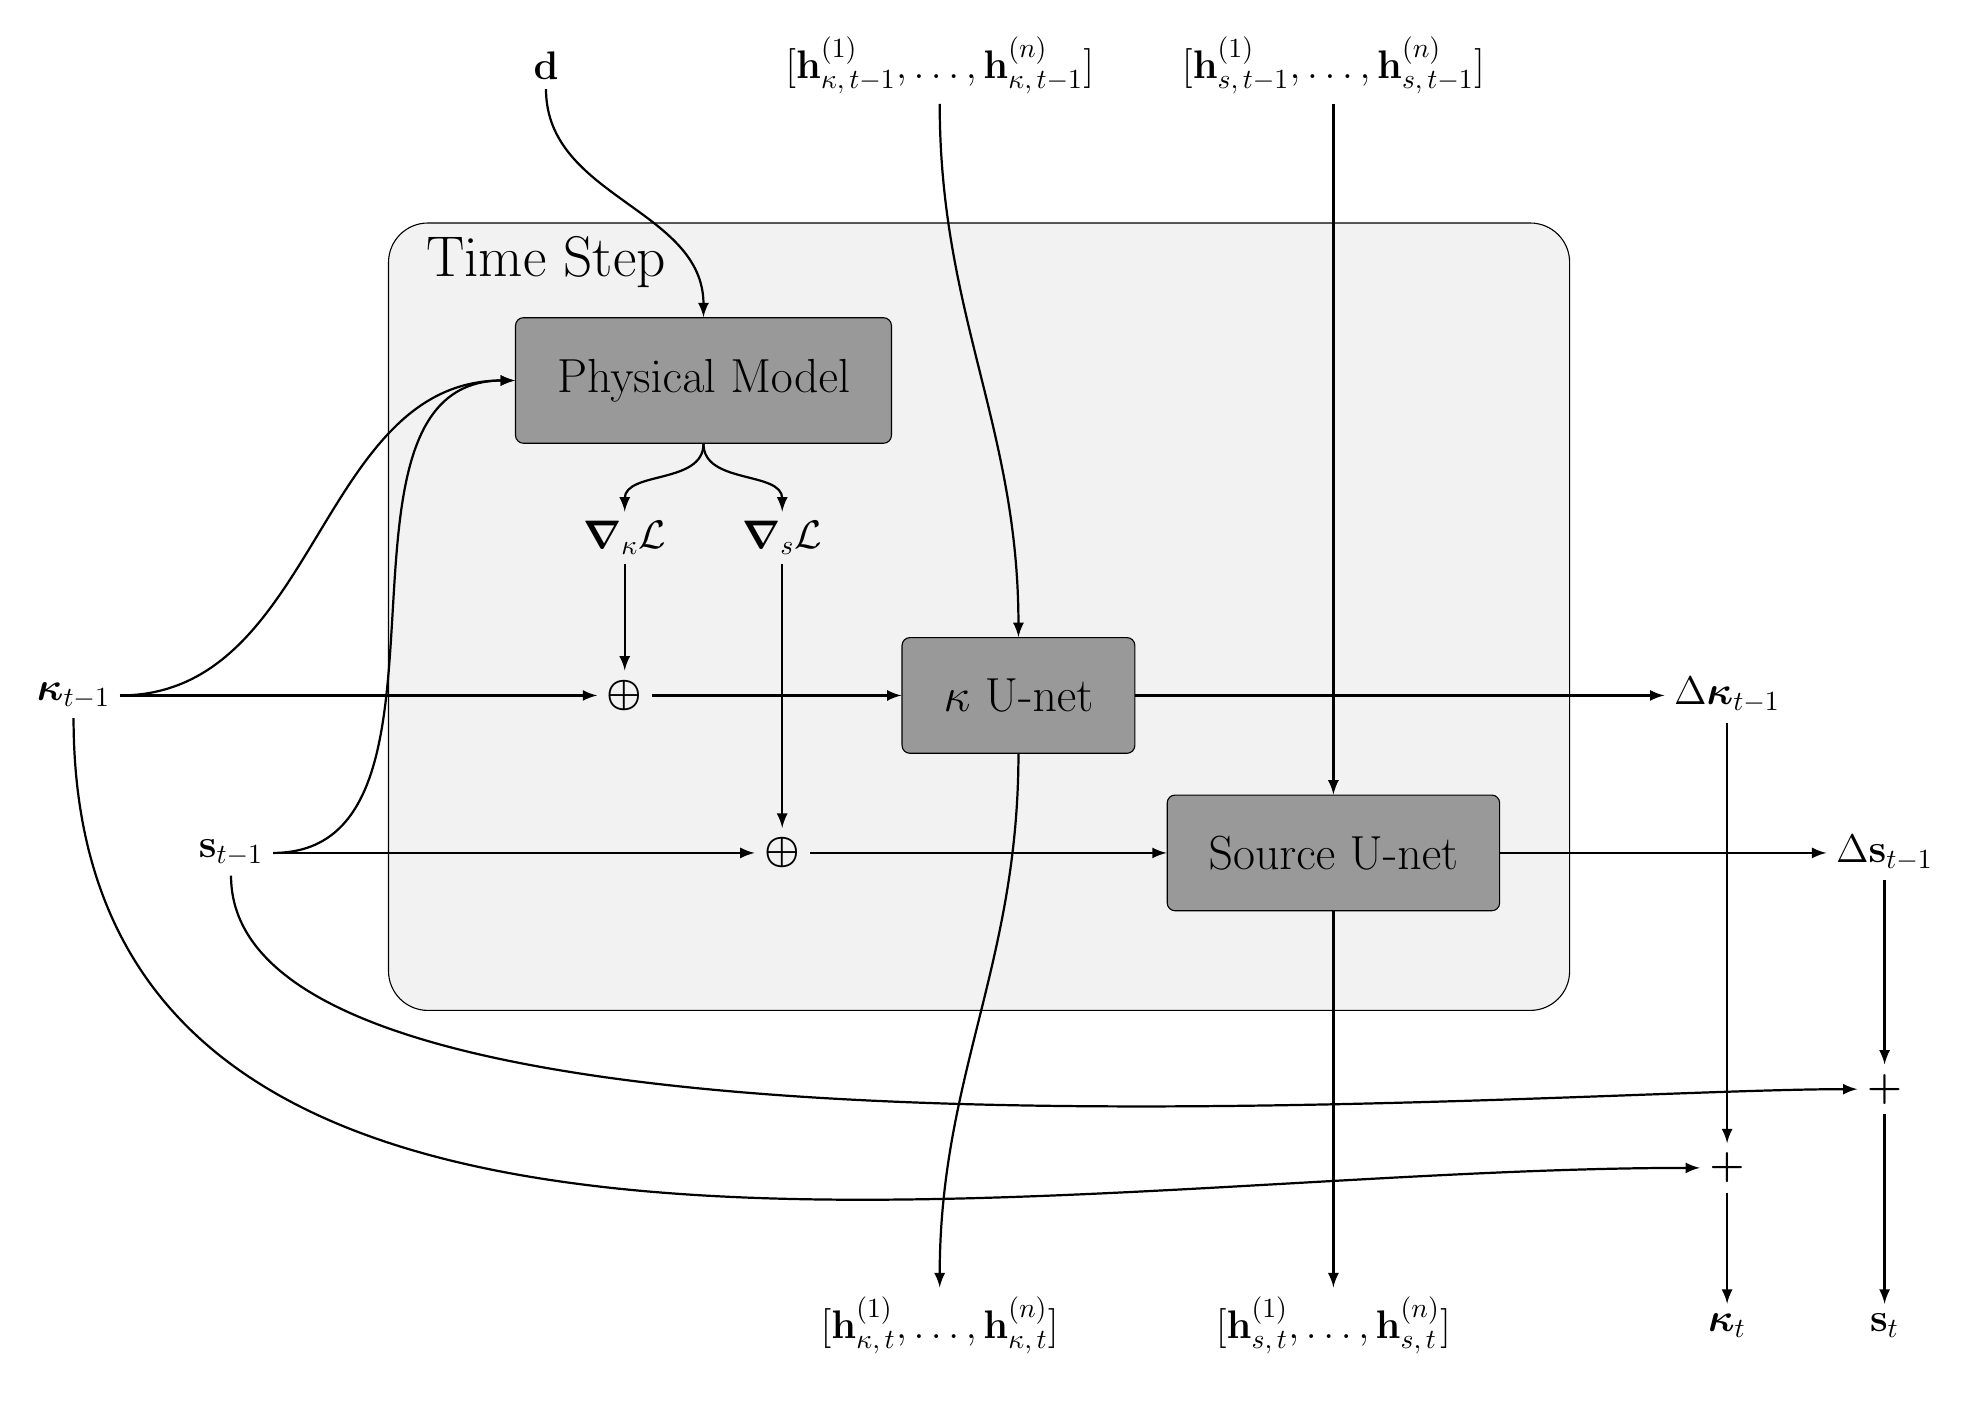
\begin{tikzpicture}[
    node distance=3cm
]
    \draw[rounded corners=0.5cm, fill=black!5, draw=black] (-5, -5) rectangle (10, 5);
    \node (title) at (-3, 4.5) {\huge Time Step};
    \node (states k) at (2, 7) {\Large $[\mathbf{h}^{(1)}_{\kappa,\, t-1}, \dots, \mathbf{h}^{(n)}_{\kappa,\, t-1}]$};
    \node (states s) at (7, 7) {\Large $[\mathbf{h}^{(1)}_{s,\, t-1}, \dots, \mathbf{h}^{(n)}_{s,\, t-1}]$};
    \node (k) at (-9, -1) {\Large $\boldsymbol{\kappa}_{t-1}$};
    \node (s) at (-7, -3) {\Large $\mathbf{s}_{t-1}$};
    \node (d) at (-3, 7) {\Large $\mathbf{d}$};
    \node[rectangle, rounded corners=0.1cm, draw=black, inner sep=15pt, fill=black!40] 
        (phys) at (-1, 3) {\LARGE Physical Model};
    \node (grad k) at (-2, 1) {\Large $\grad_{\kappa} \mathcal{L} $};
    \node (grad s) at (0, 1) {\Large $\grad_{s} \mathcal{L} $};
    \node (concat k) at (-2, -1) {\Large $\boldsymbol{\oplus}$};
    \node (concat s) at (0, -3) {\Large $\boldsymbol{\oplus}$};
    
    \node[rectangle, rounded corners=0.1cm, draw=black, inner sep=15pt, fill=black!40] 
        (unet s) at (7, -3) {\LARGE Source U-net};
    \node[rectangle, rounded corners=0.1cm, draw=black, inner sep=15pt, fill=black!40] 
        (unet k) at (3, -1) {\LARGE $\kappa$ U-net};
        
    \node (delta k) at (12, -1) {\Large $\Delta \boldsymbol{\kappa}_{t-1}$};
    \node (delta s) at (14, -3) {\Large $\Delta \mathbf{s}_{t-1}$};
    
    \node (new state k) at (2, -9) {\Large $[\mathbf{h}^{(1)}_{\kappa,\, t}, \dots, \mathbf{h}^{(n)}_{\kappa,\, t}]$};
    \node (new state s) at (7, -9) {\Large $[\mathbf{h}^{(1)}_{s,\, t}, \dots, \mathbf{h}^{(n)}_{s,\, t}]$};
    
    \node (add k) at (12, -7) {\Large $\boldsymbol{+}$};
    \node (add s) at (14, -6) {\Large $\boldsymbol{+}$};
    
    \node (new k) at (12, -9) {\Large $\boldsymbol{\kappa}_t$};
    \node (new s) at (14, -9) {\Large $\mathbf{s}_t$};

    \draw[-latex, thick, out=270, in=90] (d) to (phys);

    
    \draw[-latex, thick, out=0, in=180] (k) to (phys);
    \draw[-latex, thick, out=0, in=180] (s) to (phys);
    \draw[-latex, thick, out=270, in=90] (phys) to (grad k);
    \draw[-latex, thick, out=270, in=90] (phys) to (grad s);
    \draw[-latex, thick, out=270, in=90] (grad k) to (concat k);
    \draw[-latex, thick, out=270, in=90] (grad s) to (concat s);
    \draw[-latex, thick, out=0, in=180] (k) to (concat k);
    \draw[-latex, thick, out=0, in=180] (s) to (concat s);
    \draw[-latex, thick, out=0, in=180] (concat k) to (unet k);
    \draw[-latex, thick, out=0, in=180] (concat s) to (unet s);
    \draw[-latex, thick, out=270, in=90] (states k) to (unet k);
    \draw[-latex, thick, out=270, in=90] (states s) to (unet s);
    \draw[-latex, thick, out=0, in=180] (unet k) to (delta k);
    \draw[-latex, thick, out=0, in=180] (unet s) to (delta s);
    \draw[-latex, thick, out=270, in=90] (unet k) to (new state k);
    \draw[-latex, thick, out=270, in=90] (unet s) to (new state s);
    
    \draw[-latex, thick, out=270, in=180] (k) to (add k);
    \draw[-latex, thick, out=270, in=180, looseness=0.5] (s) to (add s);
    
    \draw[-latex, thick, out=270, in=90] (delta k) to (add k);
    \draw[-latex, thick, out=270, in=90] (add k) to (new k);
    \draw[-latex, thick, out=270, in=90] (delta s) to (add s);
    \draw[-latex, thick, out=270, in=90] (add s) to (new s);

\end{tikzpicture}
\end{document}
